
\chapter{New Demo Chapter}

\section{Sample Experiment}

				\begin{figure}[h!]
					\centering
					\begin{minipage}[b]{0.80\linewidth}
               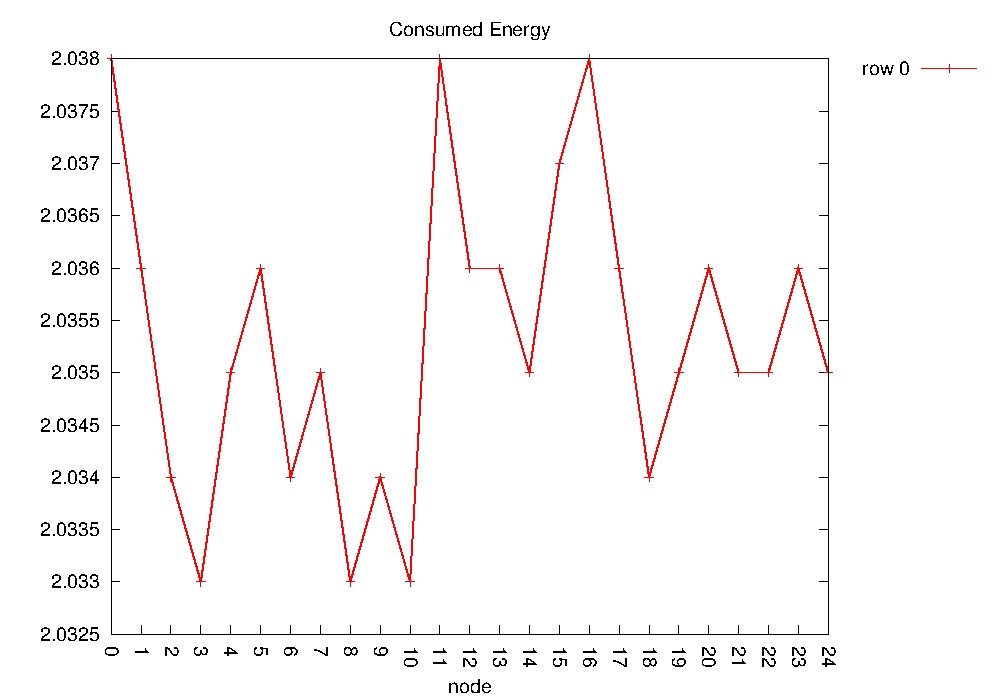
\includegraphics[scale=0.6]{demo1}
                \caption{demo figure 1}						
                \label{fig:demo1}
                \end{minipage}
                \end{figure}
                
                
     \newpage
    
 \section{Equation}    
  
  
{\bf Example Equations \cite{k3} }  
     
     \begin{equation}
  \label{eq:Continued_fractions}
  x = a_0 + \cfrac{1}{a_1
          + \cfrac{1}{a_2
          + \cfrac{1}{a_3 + \cfrac{1}{a_4} } } }
\end{equation}


\begin{equation}
  \label{eq:Multiplication}
\frac{
    \begin{array}[b]{r}
      \left( x_1 x_2 \right)\\
      \times \left( x'_1 x'_2 \right)
    \end{array}
  }{
    \left( y_1y_2y_3y_4 \right)
  }
\end{equation}


Equation \ref{eq:Continued_fractions} is a Continued fractions.\\
Equation \ref{eq:Multiplication} is Multiplication of two numbers.

%whaterver you put in $....$ will be displayed as math

$\sqrt{\frac{a}{b}}$ %this is comment, you can not cite this equation


$\sqrt[n]{1+x+x^2+x^3+\ldots}$           